\documentclass[12pt, a4paper]{article}

\usepackage[utf8]{inputenc}

% Limit the page margin to only 1 inch.
\usepackage[margin=1in]{geometry}

%Imports biblatex package
\usepackage[
backend=biber,
style=alphabetic
]{biblatex}
\addbibresource{../math-342w.bib}

% Enables the `align' environment.
\usepackage{amsmath}
\usepackage{bm}
\usepackage{array}

% Provides useful environments, such as:
% - \begin{proof} ...\end{proof}
\usepackage{amsthm}
\newtheorem{proposition}{Proposition}
\theoremstyle{definition}
\newtheorem*{definition}{Definition}
\newtheorem{theorem}{Theorem}
\newtheorem{corollary}{Corollary}

% Enables using \mathbb{}, for example \mathbb{N} for the set of natural numbers.
\usepackage{amssymb}

% Allows using letters in enumerate list environment. Use, for example:
%\begin{enumerate}[label=(\alph*)]
% ...
%\end{enumerate}
\usepackage[inline]{enumitem}

% Enable importing external graphic files and provides useful commands, like \graphicspath{}
\usepackage{graphicx}
% Images are located in a directory called "images" in the current directory.
\graphicspath{{./images/}}

% Make links look better by default.
% See: https://tex.stackexchange.com/questions/823/remove-ugly-borders-around-clickable-cross-references-and-hyperlinks
\usepackage[hidelinks]{hyperref}
\usepackage{xcolor}
\hypersetup{
	colorlinks,
	linkcolor={red!50!black},
	citecolor={blue!50!black},
	urlcolor={blue!80!black}
}

% Code Listings. Source:
% https://stackoverflow.com/questions/3175105/inserting-code-in-this-latex-document-with-indentation
\usepackage{listings}
\usepackage{color}
\usepackage[most]{tcolorbox}

\definecolor{dkgreen}{rgb}{0,0.6,0}
\definecolor{gray}{rgb}{0.5,0.5,0.5}
\definecolor{mauve}{rgb}{0.58,0,0.82}

\lstset{frame=tb,
	language=Java,
	aboveskip=3mm,
	belowskip=3mm,
	showstringspaces=false,
	columns=flexible,
	basicstyle={\small\ttfamily},
	numbers=none,
	numberstyle=\tiny\color{gray},
	keywordstyle=\color{blue},
	commentstyle=\color{dkgreen},
	stringstyle=\color{mauve},
	breaklines=true,
	breakatwhitespace=true,
	tabsize=3
}

\newcommand{\prob}{\text{P}}
%\newcommand{\complement}{\mathsf{c}}
\title{Lecture 14: MATH 342W: Introduction to Data Science and Machine Learning}
\author{Sergio E. Garcia Tapia\thanks{Based on lectures of Dr. Adam Kapelner at Queens College.
See also the \href{https://github.com/kapelner/QC_MATH_342W_Spring_2025}{course GitHub page}.}}
\date{March 28, 2025 (last updated \today)}

\begin{document}
	\maketitle
	\section*{Polynomial Regression}
	Let $\mathcal{Y}=\mathbb{R}$ and $p=1$. In our framework, we have
	\begin{align*}
		y = g(\bm{x}) + 
		\underbrace{(h^*(\bm{x}) - g(\bm{x}))}_{{\text{estimation}}} + 
		\underbrace{f(\bm{x}) - h^*(\bm{x})}_{\textit{misspecification}} +
		\underbrace{t(\bm{z}) - f(\bm{x})}_{\textit{ignorance}}
	\end{align*}
	We have learned that we can decrease estimation error by increasing $n$ relative
	to $p$. Reducing ignorance error requires us to gather more features. Unfortunately,
	that is usually not within the scope of our work. In practice, we are in control
	of estimation and misspecification error, but today our focus will be on the latter.
	The focus of this course is slowly shifting towards machine learning.
	
	
	\begin{figure}
		\centering
		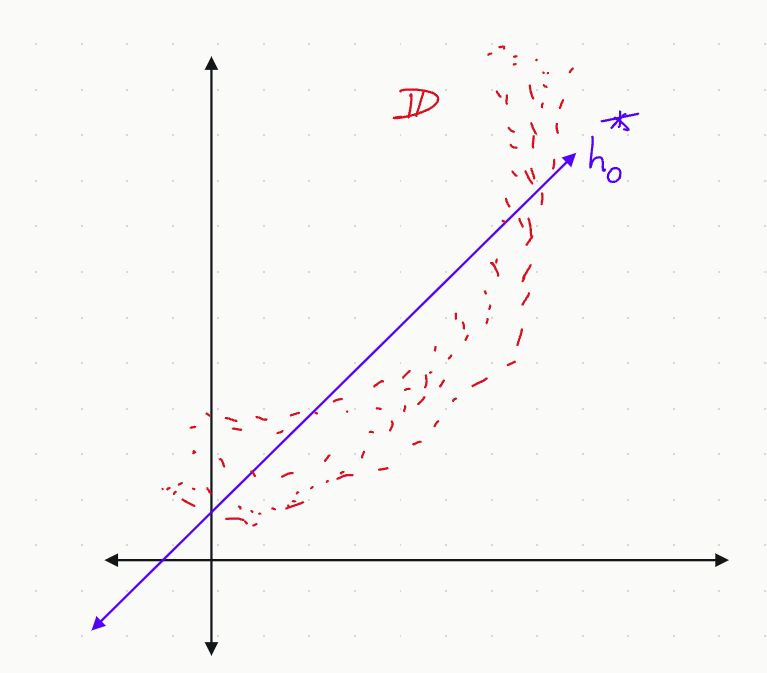
\includegraphics[width=0.4\textwidth]{underfit-with-linear-function}
		\caption{Underfitting a data set $\mathbb{D}$ with a linear approximation
		$h_0^*$.}
		\label{fig:underfit-D-with-linear}
	\end{figure}
	
	Consider the data set $\mathbb{D}$ depicted in Figure~\ref{fig:underfit-D-with-linear}
	and the linear approximation $h_0*$ depicted, where $h_0\in \mathcal{H}_0$ and
	\begin{align*}
		\mathcal{H}_0 =\{\, w_0+w_1x \mid w_0,w_1\in \mathbb{R}\,\} 
	\end{align*}
	We know that $h_0^*$ is the best possible approximation to $f$ in $\mathcal{H}_0$, where
	$f$ is in turn the best approximation to $t$ with the features that we are using as proxies
	to the true drivers.
	
	We reiterate that $h_0^*$ is likely not close to $f$, but it is the best we can do in
	$\mathcal{H}_0$; simply, $f(x)$ is \textit{not} linear in this this example, so
	even the best linear approximation will not perform well. This is an example of
	\textbf{underfitting}.
	
	Let's allow for a more \textit{expansive} (larger) candidate set, an expanded
	\textbf{functional basis}. Consider:
	\begin{align*}
		\mathcal{H} = \{\, w_0 + w_1x + w_2x^2 \mid w_0,w_1,w_2\in\mathbb{R}\,\}
	\end{align*}
	which includes a quadratic term, allowing us to fit parabolas and lines, and
	linear combinations of parabolas and lines. With this candidate set,
	we can better fit $f(x)$, reducing misspecification.
	\begin{figure}
		\centering
		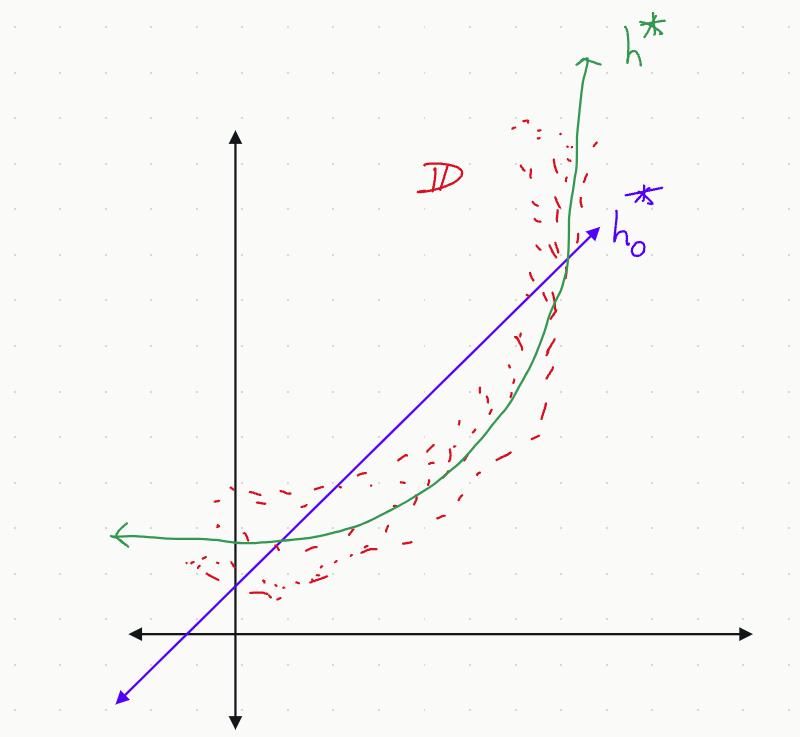
\includegraphics[width=0.4\textwidth]{better-fit-with-quadratic-function}
		\caption{Underfitting a data set $\mathbb{D}$ with a linear approximation
			$h_0^*$.}
		\label{fig:better-fit-D-with-quadratic}
	\end{figure}
	Figure~\ref{fig:better-fit-D-with-quadratic} shows fitting $\mathbb{D}$ with
	a quadratic function $h^*\in \mathcal{H}$. Note how the coefficient $w_2$
	of the quadratic term of the functions in $\mathcal{H}$ are a scalar
	multiple of $x^2$, which is the square of the single feature we have.
	That is, we still only measure 1 feature, but we are using it twice. In this
	setting, we say $p_{\text{raw}} = 1$, and $p=2$; we call $x^2$ a \textbf{transformed}
	or \textbf{derived} feature. Compare this with using a linear model, where we
	would introduce a new coefficient $b_2$, but in that case, it would be an example
	of chance capitalization, and hence overfitting.
	
	Using derived features that are squares, cubes, etc, of the raw features is an example
	of \textbf{polynomial regression}. Here's a question: is
	\begin{align*}
		\hat{y} = b_0 + b_1x + b_2 x^2
	\end{align*}
	a linear model? We can justify the answer both ways:
	\begin{itemize}
		\item \textbf{Yes}: It is linear because $g$ is a linear combination of the
		raw and derived features.
	\item \textbf{No}: It is not linear because $g$ is not a straight line (hyperplane).	\end{itemize}
	Now, we may ask whether it is justified or ``principled" to use polynomial regression.
	In fact, it is, and it s a consequence of the famous Stone-Weierstrass theorem, which
	proves that any continuous function $f:\mathbb{R}^p\to \mathbb{R}$ can be approximated
	by a sum of polynomials. If you have learned basic calculus, you may have seen a similar
	example of this: Taylor's Theorem. Indeed, Taylor Theorem says that an infinitely differentiable
	function can be expressed as an infinite sum of polynomials. However, Stone-Weierstrass
	does not require differentiability, only continuity.
	
	How do we find $g\in \mathcal{H}$ in the case of polynomial regression? Suppose
	we have $\mathbb{D}=\{(x_1,y_1),(x_2,y_2),\ldots,(x_n,y_n)\}$. Then we can
	transform our matrix of raw features into a design matrix $X$ that has the
	derived features used in quadratic regression:
	\begin{align*}
		X_{\text{raw}} = \begin{bmatrix}
			x_1\\
			x_2\\
			\ldots\\
			x_n
		\end{bmatrix}
		\quad
		\implies
		\quad
		X = \begin{bmatrix}
			1 & x_1 & x_1^2\\
			1 & x_2 & x_2^2\\
			\vdots & \vdots & \vdots\\
			1 & x_n & x_n^2
		\end{bmatrix}
	\end{align*}
	In the R programming language, which would simply be:
	\begin{lstlisting}[language=R]
X = cbind(1, x, x^2)
	\end{lstlisting}
	Then we can \textit{apply OLS using matrix $X$, just like before}:
	\begin{align*}
		\bm{b} &:= (X^\top X)^{-1}X^\top \bm{y}\\
		\bm{e} &:= \bm{y} - \bm{\hat{y}} = \bm{y} - X\bm{b}\\
		SSE &:= \|\bm{e}\|^2\\
		MSE &:= \frac{SSE}{n - (p + 1)}\\
		RMSE &:= \sqrt{MSE}\\
	\end{align*}
	Note that we are making a tradeoff. By allowing a quadratic term, our
	misspecification error increases, but our estimation error increases also.
	If $p+1\lll n$, then increasing $p$ via these derived features may
	be justified if the misspecification error decreases meaningfully.
	\subsection*{The Design Matrix with Transformed Features}
	One concern we need to address is whether the matrix $X$ obtained from
	$X_{\text{raw}}$ is full rank after adding the new column whose entries
	are squares of the raw feature. One way to justify it is as follows.
	Suppose that the columns are linearly dependent. Then there are coefficients
	$c_0,c_1,c_2$ making up a vector $\bm{c}=\begin{bmatrix}
		c_0 & c_1 & c_2
	\end{bmatrix}^\top\in\mathbb{R}^3$
	such that $X\bm{c}=\bm{0}_{n \times 1}$. If we define a polynomial $p(x)=c_0+c_1x+c_2x^2$,
	then
	\begin{align*}
		\begin{bmatrix}
			0\\
			0\\
			\vdots\\
			0
		\end{bmatrix}
		=
		\bm{0}_{n\times 1}
		=
		X\bm{c}
		=
		\begin{bmatrix}
			1 & x_1 & x_1^2\\
			1 & x_2 & x_2^2\\
			\vdots & \vdots & \vdots\\
			1 & x_n & x_n^2
		\end{bmatrix}
		\begin{bmatrix}
			c_0\\
			c_1\\
			c_2
		\end{bmatrix}
		=\begin{bmatrix}
			c_0 + c_1x_1^2 + c_2x_1^2\\
			c_0 + c_2x_2^2 + c_2x_2^2\\
			\vdots\\
			c_0 + c_1x_n^2 + c_2x_n^2
		\end{bmatrix}
		=\begin{bmatrix}
			p(x_1)\\
			p(x_2)\\
			\vdots\\
			p(x_n)
		\end{bmatrix}
	\end{align*}
	Hence, $p(x_1)=p(x_2)=\cdots=p(x_n)=0$. However, since $p$ is a polynomial of degree
	two, it has at most 2 zeroes. Therefore, if at least $3$ distinct values for the feature
	$x$ exist in $\mathbb{D}$, it's impossible for $p$ to be zero on all of them.
	In general we deal with $p + 1 \lll n$, so that we can usually guarantee
	$X$ is full rank.
	
	In particular, if $X$ has binary features (that is, its values can be only $0$
	and $1$), then we cannot apply this transformation, since squaring will result
	in the same value, hence yielding a linearly dependent column.
	\subsection*{Interpretability and Machine Learning}
	One point is whether our new result is interpretable, and how much that
	matters to us. Consider
	\begin{align*}
		\hat{y} = b_0 + b_1x + b_2x^2 = b_0 + (b_1 + b_2x)x
	\end{align*}
	We can say that if $x$ changes by $1$, then $\hat{y}$ changes by $b_1+b_2x$.
	What if we go further, fitting a cubic?
	\begin{align*}
		\hat{y} = g(x) = b_0 + b_1x + b_2x^2 + b_3x^3
	\end{align*}
	As we fit higher degree polynomials, we lose easy the interpretation
	that we get from a linear model (and quadratic to a lesser extent).
	However, we do get a closer fit. The tradeoff is interpretability and
	model complexity.
	
	This matters in machine learning, which we now define.
	\begin{tcolorbox}[breakable]
		\begin{definition}[Machine Learning]
			Machine learning is supervised learning (some people stop here),
			with a very flexible $\mathcal{H}$.
		\end{definition}
	\end{tcolorbox}
	A downside of a very flexible $\mathcal{H}$ is the loss of interpretability.
	\section*{Interpolation and Extrapolation}
	\begin{tcolorbox}[breakable]
		\begin{definition}
			\label{dfn:range-X-rectangle}
			Given design matrix $X$, we define the \textbf{range of $X$}
			to be a rectangle in $\mathbb{R}^{p}$:
			\begin{align*}
				\text{Range}[X] =
				[X_{\cdot 1,\text{min}}, X_{\cdot 1,\text{max}}] \times
				[X_{\cdot 2,\text{min}}, X_{\cdot 2,\text{max}}] \times
				\cdots \times
				[X_{\cdot p,\text{min}}, X_{\cdot p,\text{max}}]
			\end{align*}
			Here, $\times$ is used to denote a Cartesian product, $X_{\cdot, j}$
			denotes the $j$th column of $X$ (containing all $n$ instances of the
			$j$th feature), and $[X_{\cdot j,\text{min}}, X_{\cdot j,\text{max}}]$
			denotes a closed interval in $\mathbb{R}$, delimited by the smallest value of
			the $j$th feature and the largest value of the $j$ feature in $X$
			(see Figure~\ref{fig:range-X-rectangle}).
		\end{definition}
	\end{tcolorbox}
	\begin{figure}
		\centering
		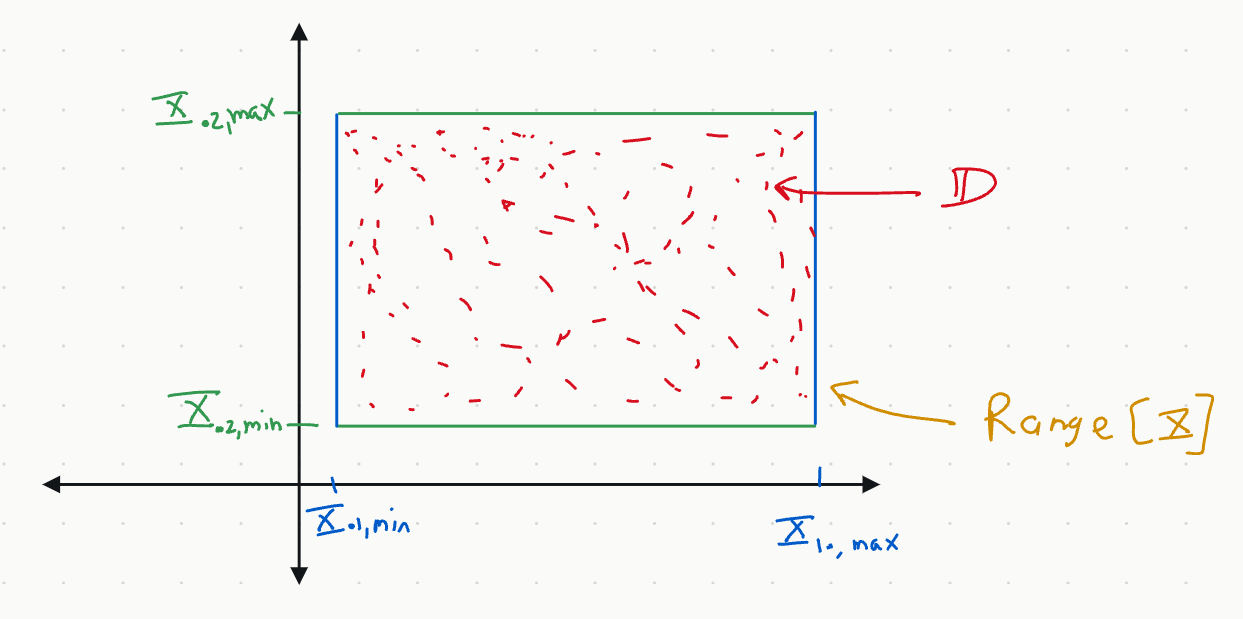
\includegraphics[width=0.7\textwidth]{range-X-rectangle}
		\caption{A depiction of the range of $X$, as described in
			 Definition~\ref{dfn:range-X-rectangle}.}
	 	\label{fig:range-X-rectangle}
	\end{figure}
	\begin{tcolorbox}[breakable]
		\begin{definition}
			\label{ref:interpolation-extrapolation}
			Given a design matrix $X$:
			\begin{itemize}
				\item \textbf{Interpolation} is predicting for $\bm{x}\in \text{Range}[X]$.
				\item \textbf{Extrapolation} is predicting for $\bm{x}\notin \text{Range}[X]$.
			\end{itemize}
		\end{definition}
	\end{tcolorbox}
	An important fact to remember is that models are defined for \textit{interpolation},
	and bad things happen during extrapolation. Interestingly, different candidate
	sets $\mathcal{H}$ and different algorithms $\mathcal{A}$ lead to different
	behavior under extrapolation.
	\section*{Logarithmic Approximations}
	At times, it can be useful to perform a transformation on the response and (or)
	the feature values. A popular such transformation is a \textit{logarithmic
	transformation}. First, recall the following Taylor series approximation:
	\begin{align*}
		\ln(1 + x) = x - \frac{x^2}{2}+\frac{x^3}{3} -\cdots+\cdots \approx x,\quad \text{if }x\approx 0
	\end{align*}
	Therefore,
	\begin{align}
		\ln((1 + x) - 1)\approx x-1 \label{eqn:lnx-taylor-approx}
	\end{align}
	We will apply (\ref{eqn:lnx-taylor-approx}) in the following discussion.
	\subsection*{$\hat{y}$ vs $\log(x)$}
	Now suppose we transform a feature $x$ into $\ln(x)$, and apply OLS, yielding
	the model
	\begin{align*}
		\hat{y} = b_0 + b_1\ln(x)
	\end{align*}
	We want to try to interpret what happens if $x$ changes. Let $\Delta x := x_f - x_0$,
	where $x_0$ is the initial value of $x$ and $x_f$ is the final value of $x$
	after some change. Then the change in the prediction $\hat{y}$ is:
	\begin{align*}
		\Delta \hat{y} &= (b_0 + b_1\ln(x_f)) - (b_0 + b_1\ln(x_0))\\
		&=b_1(\ln(x_f) - \ln(x_0))\\
		&=b_1\ln \left(\frac{x_f}{x_0}\right)\\
		&\approx b_1\left(\frac{x_f}{x_0} - 1\right)
		\tag{by (\ref{eqn:lnx-taylor-approx})}\\
		&=b_1\underbrace{\left(\frac{x_f-x_0}{x_0}\right)}_{\text{proportional change}}
	\end{align*}
	We can interpret this as follows: if $x$ increases by $27\%$, then the predicted response
	increases by $b_1\cdot 27\%$.
	\subsection*{$\log(\hat{y})$ vs $x$}
	Next, suppose we transform the response into $\ln(y)$ and leave the feature $x$
	unchanged:
	\begin{align*}
		\ln(\hat{y}) = b_0 + b_1x
	\end{align*}
	Then if $x$ changes by $\Delta x = x_f-x_0$, the corresponding change in the $\ln(\hat{y})$
	is
	\begin{align*}
		\Delta \ln(\hat{y})=
		&=\ln(\hat{y}_f) - \ln(\hat{y}_0)\\
		&= (b_0 + b_1x_f) - (b_0 + b_1x_0)\\
		&=b_1\Delta x
	\end{align*}
	Hence,
	\begin{align*}
	b_1\Delta x
	&= \ln\left(\frac{\hat{y}_f}{\hat{y}_0}\right)\\
	&\approx \frac{\hat{y}_f - \hat{y}_0}{\hat{y}_0}
	\tag{by (\ref{eqn:lnx-taylor-approx})}
	\end{align*}
	The interpretation is that if there is a one unit change in $x$, then the predicted
	response is a $b_1$ proportion change. For example, if $b_1=0.37$, then
	$\hat{y}$ changes by $37\%$.
	\subsection*{$\log(y)$ vs $\log(x)$}
	Suppose we transform both the feature and the response by applying the logarithm:
	\begin{align*}
		\ln(\hat{y}) = b_0 + b_1\ln(x)
	\end{align*}
	Then a similar calculation yields
	\begin{align*}
		\frac{\hat{y}_f - \hat{y}_0}{\hat{y}_0} \approx b_1 \frac{x_f - x_0}{x_0}
	\end{align*}
	Let $b_1 \approx 0.37$. If $x$ increases by $27\%$, then the predicted response
	increases by $0.37\cdot 0.27\cdot 100$ percent.
	\subsection*{Summary on Transformations}
	Usually, transformations are done on the features (the $x$'s). We saw one example
	in which we transform the response $y$ to $\ln(y)$. In fact, the
	most common transformations for $\mathcal{Y}=\mathbb{R}$ are $\ln$,
	$\log_{10}$, and $\log_{2}$. Note that doing this amounts to the following:
	\begin{align*}
		\bm{y} = \begin{bmatrix}
			y_1\\
			y_2\\
			\vdots\\
			y_n
		\end{bmatrix}
		\quad
		\implies
		\quad
		\bm{y}'
		\begin{bmatrix}
			\ln(y_1)\\
			\ln(y_2)\\
			\vdots\\
			\ln(y_3)
		\end{bmatrix}
	\end{align*}
	and then using OLS as usual with $\bm{y} = (X^\top X)^{-1}X^\top \bm{y}'$.
	This yields
	\begin{align*}
		\ln(\hat{y})
		&= b_0 + b_1 x_1 + \cdots + b_px_p \iff\\
		\hat{y} &= e^{b_0} e^{b_1x_1}\cdots e^{b_px_p}\\
		&=e^{b_0}(e^{b_1})^{x_1}\cdots )(e^{b_p})^{x_p}\\
		&=m_0\cdot m_1^{x_1}\cdots m_p^{x_p}
	\end{align*}
	which becomes a multiplicative model. We can do this, but we must bear in mind
	that the units of the response change. Thus, we eventually must reverse the
	transformation. Indeed, we cannot compare the response of the original model with
	that of the transformed model, because the units do not match. We could use $R^2$
	since it is unitless, but since the $R^2$ metric is hard to interpret, it
	is often not as useful.
	
	Another thing to bear in mind is that if we apply a logarithmic transformation,
	then a small residual in the logarithmic change can still indicate a large error in
	the original units, because we must apply the exponential function to reverse
	it.
	
	In summary, we can transform the response, as long as we are careful about the units
	of the predictions, the error metrics, and how we compare model fits.
	
	One good reason to perform a transformation is that $y$ may be right-skewed,
	which can make it difficult to capture extremes, as depicted in
	Figure~\ref{fig:histogram-y-difficult-capturing-extremes}.
	\begin{figure}
		\centering
		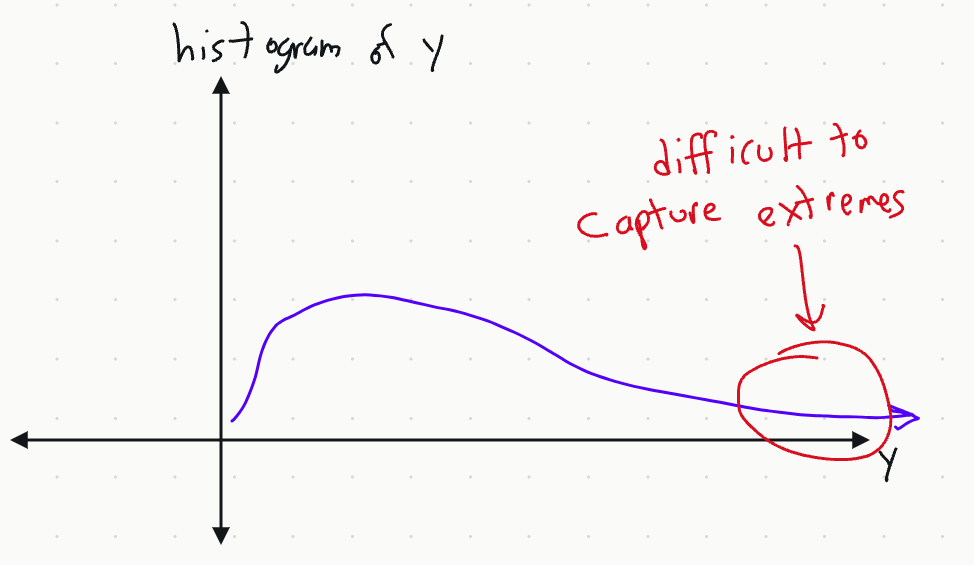
\includegraphics[width=0.5\textwidth]{histogram-y-capturing-extremes}
		\caption{A histogram of the responses values $y$.}
		\label{fig:histogram-y-difficult-capturing-extremes}
	\end{figure}
	
	Applying a logarithmic transformation results in something like in
	Figure~\ref{fig:log-transformation-histogram-y}.
	\begin{figure}
		\centering
		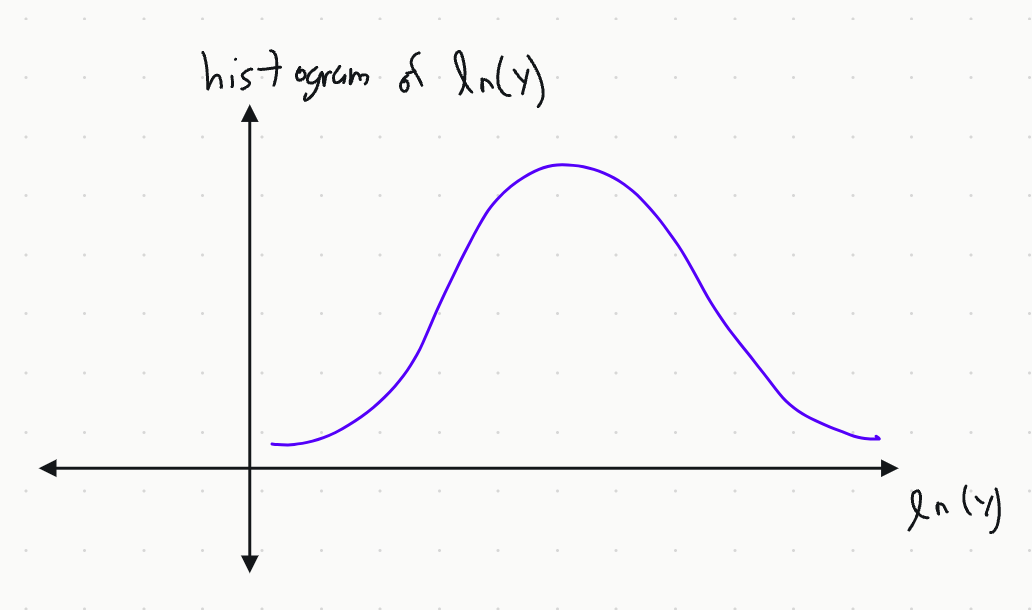
\includegraphics[width=0.5\textwidth]{log-transformation-histogram-y}
		\caption{A logarithmic transformation applied to the response $y$
		from Figure~\ref{fig:histogram-y-difficult-capturing-extremes}}.
		\label{fig:log-transformation-histogram-y}
	\end{figure}
	\section*{Generalized Additive Model (GAM)}
	Imagine adding many transformations to your design matrix $X$. For example,
	polynomial, logarithmic, trigonometric functions, etc. Your model may look
	like
	\begin{align*}
		g(\bm{x}) = g_1(x_1) + g_2(x_2) +\cdots+g_p(x_p)
	\end{align*}
	where the $g_j$'s are arbitrarily complex and possibly non-linear (note that
	in simple polynomial regression, we have $g_j(x)=x^j$). This is called a
	\textbf{generalized linear model (GAM)}. Although well-studied, GAMs have
	fallen out of favor, as we will see when we discuss random forests.
	
	What is missing from this type of model $\mathcal{H}$? Functions of multiple
	variables.
	Notice that functions of multiple variables are missing from the type of
	model $\mathcal{H}$ implied by GAM, so we have
	\begin{align*}
		\frac{\partial}{\partial x_\ell} [g_j(x_j)] = 0,\quad \forall_{j\neq \ell}
	\end{align*}
	Put another way, the model does not account for \textit{interactions between features}.
	The following model for $p=2$ allows for a \textit{first-order interaction}:
	\begin{align*}
		\mathcal{H} = \{\,
		w_0 + w_1x + w_2x_2 + w_3x_1x_2 \mid \bm{w}\in \mathbb{R}^4
		\,\}
	\end{align*}
	Here, $x_1$ interacts with $x_2$, and the transformation from $X_\text{raw}$ is
	\begin{align*}
		X_\text{raw} = \begin{bmatrix}
			x_{11} & x_{22}\\
			x_{12} & x_{22}\\
			\vdots & \vdots\\
			x_{1n} & x_{2n}
		\end{bmatrix}
		\quad
		\implies
		\quad
		X = \begin{bmatrix}
			1 & x_{11} & x_{21} & x_{11} x_{21}\\
			1 & x_{12} & x_{22} & x_{12} x_{22}\\
			\vdots & \vdots & \vdots & \vdots\\
			1 & x_{1n} & x_{2n} & x_{1n}x_{2n}
		\end{bmatrix}
	\end{align*}
	Again, we apply OLS to get $\bm{b} = (X^\top X)^{-1}X^\top \bm{y}$.
	This time, we prediction is given by
	\begin{align*}
		\bm{y}
		&= b_0 + b_1x_1 + b_2x_3 + b_3x_1x_2\\
		&= b_0 + b_1x_1 + (b_2 + b_3x_1)x_2\\
		&= b_0 + b_2x_2 + (b_1 + b_3x_2)x_1
	\end{align*}
	We can interpret it the following way:
	\begin{itemize}
		\item If $x_2$ increases by $1$ unit, then $\hat{y}$ changes by $b_2+b_3x_1$.
		\item If $x_1$ increases by $1$ unit, then $\hat{y}$ changes by $b_1+b_3x_2$.
	\end{itemize}
	\pagebreak
	\printbibliography
\end{document}